\documentclass{article} % For LaTeX2e
\usepackage{nips14submit_e,times}
\usepackage{amsmath}
\usepackage{amsthm}
\usepackage{amssymb}
\usepackage{mathtools}
\usepackage{hyperref}
\usepackage{url}
\usepackage{algorithm}
\usepackage[noend]{algpseudocode}
%\documentstyle[nips14submit_09,times,art10]{article} % For LaTeX 2.09

\usepackage{mathrsfs}
\usepackage{graphicx}
\usepackage{caption}
\usepackage{subcaption}

\def\eQb#1\eQe{\begin{eqnarray*}#1\end{eqnarray*}}
\def\eQnb#1\eQne{\begin{eqnarray}#1\end{eqnarray}}
\providecommand{\e}[1]{\ensuremath{\times 10^{#1}}}
\providecommand{\pb}[0]{\pagebreak}

\newcommand{\E}{\mathrm{E}}
\newcommand{\Var}{\mathrm{Var}}
\newcommand{\Cov}{\mathrm{Cov}}

\def\Qb#1\Qe{\begin{question}#1\end{question}}
\def\Sb#1\Se{\begin{solution}#1\end{solution}}

\newenvironment{claim}[1]{\par\noindent\underline{Claim:}\space#1}{}
\newtheoremstyle{quest}{\topsep}{\topsep}{}{}{\bfseries}{}{ }{\thmname{#1}\thmnote{ #3}.}
\theoremstyle{quest}
\newtheorem*{definition}{Definition}
\newtheorem*{theorem}{Theorem}
\newtheorem*{lemma}{Lemma}
\newtheorem*{question}{Question}
\newtheorem*{preposition}{Preposition}
\newtheorem*{exercise}{Exercise}
\newtheorem*{challengeproblem}{Challenge Problem}
\newtheorem*{solution}{Solution}
\newtheorem*{remark}{Remark}
\usepackage{verbatimbox}
\usepackage{listings}
\title{Linear Algebra II: \\
Problem Set I}


\author{
Youngduck Choi \\
CIMS \\
New York University\\
\texttt{yc1104@nyu.edu} \\
}


% The \author macro works with any number of authors. There are two commands
% used to separate the names and addresses of multiple authors: \And and \AND.
%
% Using \And between authors leaves it to \LaTeX{} to determine where to break
% the lines. Using \AND forces a linebreak at that point. So, if \LaTeX{}
% puts 3 of 4 authors names on the first line, and the last on the second
% line, try using \AND instead of \And before the third author name.

\newcommand{\fix}{\marginpar{FIX}}
\newcommand{\new}{\marginpar{NEW}}

\nipsfinalcopy % Uncomment for camera-ready version

\begin{document}


\maketitle

\begin{abstract}
This work contains solutions to the problem set I
of Linear Algebra II 2016 at Courant Institute of Mathematical Sciences.
\end{abstract}

\bigskip

\begin{question}[1]
\hfill
\begin{figure}[h!]
  \centering
    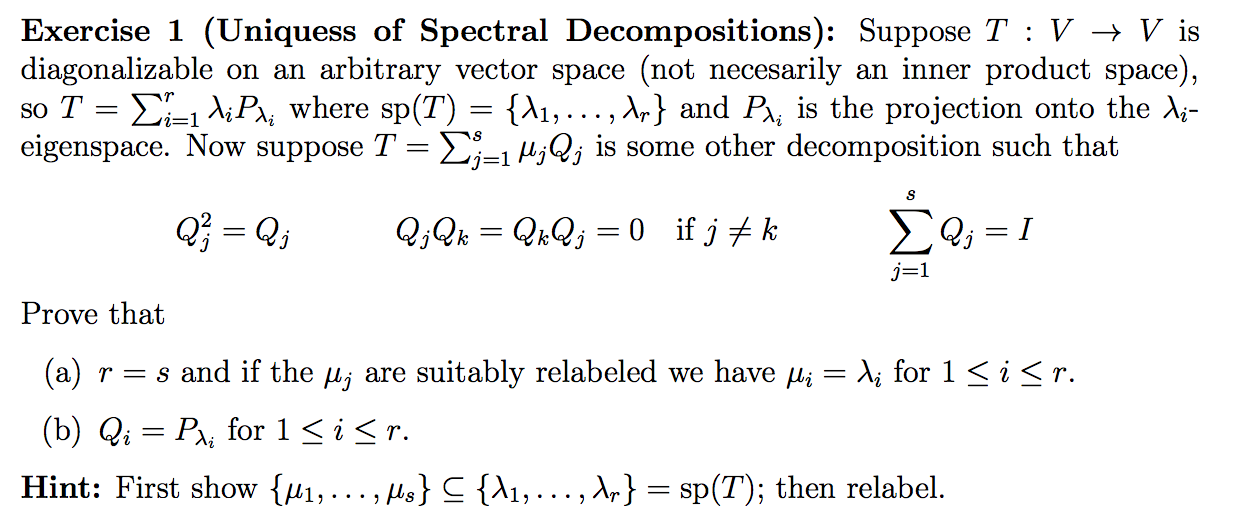
\includegraphics[width=1\textwidth]{LA-2-1.png}
\end{figure}
\end{question}
\begin{solution}
\textbf{((a)} 
Firstly, note that $u_j$ is an eigenvalue of $T$. To see this, let $v \neq 0 \in Q_j$.
Then, as $Q_jv = v $, it follows that
\eQb
Tv &=& \sum_{i=1}^{s} u_i Q_i v \\
&=& \sum_{i=1}^{s} u_i Q_i Q_j v \\
&=& u_j Q_j^2 v \\
&=& u_j v .
\eQe
Therefore, we have shown that $\text{Im}(Q_j) \subset \text{Im}(P_{u_j})$. Next, suppose $w$
is an arbitrary eigenvector of $T$, It follows that $w = \sum_{i=1}^{s} Q_i w$, which
expresses $w$  as a sum of zero-vectors and eigenvectors. But, since eigenvectors corresponding
to distinct eigenvalues are linearly independent, the only possibility is that 
$w \in \text{Im}(Q_i) = \text{Im}(P_{\lambda_i})$ for some $i$. Hence, we have shown that
\eQb
\{ u_1,..,u_r\} = \text{sp}(T).
\eQe

\newpage

\textbf{(b)} We have shown that $\text{Im}(Q_i) = \text{Im}(P_{\lambda_i})$ for all $i$ after
relabeling. As they are both projections, the proof of uniqueness will be established, if 
we show that they possess the same kernel. By assumption, we have
\eQb
\text{ker}(P_{\lambda_i}) &=& \sum_{j \neq i} \text{Im}(P_{\lambda_j}) \\
&=& \sum_{j \neq i} \text{Im}(Q_j). \\ 
\eQe
Let $v \in \text{ker}(P_{\lambda_i})$. Then, it follows that 
\eQb
v &=& \sum_{j \neq i } Q_j x_j \\
\eQe
for $x_j \in V$ with $j \neq i$. Furthermore, we have
\eQb
Q_i v &=& Q_i \sum_{j \neq i} Q_j x_j = 0 .
\eQe
Converse holds true with the same logic. 
\hfill $\qed$
\end{solution}

\newpage

\begin{question}[2]
\hfill
\begin{figure}[h!]
  \centering
    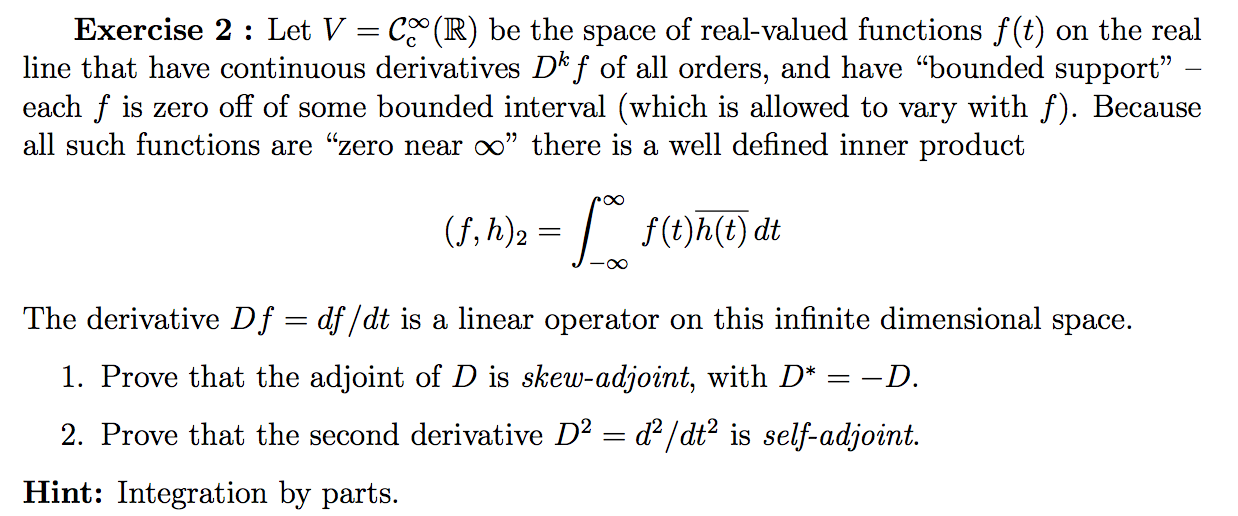
\includegraphics[width=1\textwidth]{LA-2-2.png}
\end{figure}
\end{question}
\begin{solution}
\textbf{(a)} Let $f,g \in V$. By integration by parts, we have
\eQb
\int_{-\infty}^{\infty} Df \overline{g} dt + \int_{-\infty}^{\infty} f \overline{Dg} dt
&=& [f\overline{g}]_{-\infty}^{\infty} \\
&=& 0, 
\eQe
as $f,g$ have bounded supports. Therefore, it follows that
\eQb
(Df,g) &=& -(f,Dg).
\eQe
Since $f,g$ were arbitrary, we have shown that $D^* = D$.

\bigskip

\textbf{(b)} By $(a)$, we have
\eQb
(D^2f,g) &=& -(Df,Dg) \\
&=& (f,D^2g), 
\eQe
for $f,g \in V$. Therefore, $D^2$ is self-adjoint. \hfill $\qed$


\end{solution}

\newpage

\begin{question}[3]
\hfill
\begin{figure}[h!]
  \centering
    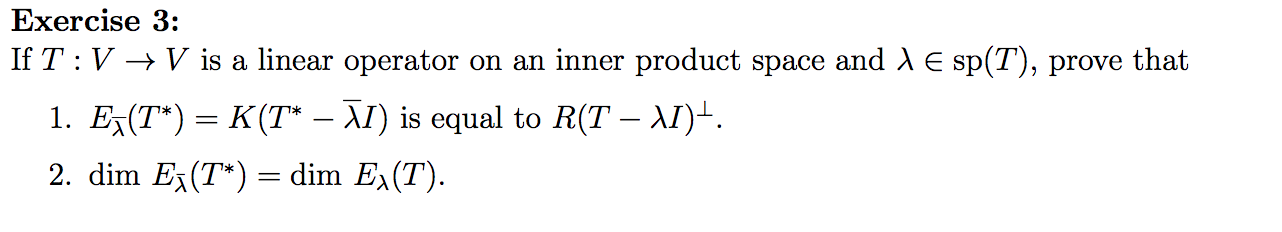
\includegraphics[width=1\textwidth]{LA-2-3.png}
\end{figure}
\end{question}
\begin{solution}
\textbf{(1)} We first claim that for $K(T^*) = R(T)^{\perp}$. We prove it by showing the
following series of equivalence. 
\eQb
w \in K(T^*) &\iff& T^* w = 0 \\
&\iff& <v, T^* w> = 0 \>\>\> \forall v \in V \\
&\iff& <Tv, w> = 0 \>\>\> \forall v \in V \\
&\iff& w \in R(T)^{\perp},
\eQe
as required.
Now, by the elementary properties of adjoint, it follows that 
\eQb
(T - \lambda I)^* &=& T^* - (\lambda I)^* \\
&=& T^* - \overline{\lambda} I^* \\
&=& T^* - \overline{\lambda} I.
\eQe
Therefore, combining the two results together, we have shown that
\eQb
E_{\overline{\lambda}}(T^*) &=& R(T - \lambda I)^{\perp} \\
\eQe


\bigskip

\textbf{(2)} By definition of eigenspace, and the rank-nullity theorem, we have
\eQb
\text{dim} E_{\lambda}(T) &=& \text{dim} N(T - \lambda I) \\
&=& \text{dim}V - \text{dim} R(T - \lambda I).
\eQe
As a subspace of a linear space forms a direct sum with its orthogonal complement, we have
that
$\text{dim}R(T-\lambda I) = \text{dim}V - \text{dim}R(T-\lambda I)^{\perp}$. By $(1)$,
it follows that 
$\text{dim}R(T-\lambda I) = \text{dim}V - 
\text{dim}E_{\overline{\lambda}}(T^{*})$.
Substituting to the result to the previous equation, we obtain 
\eQb
\text{dim} E_{\lambda}(T) &=&
\text{dim}E_{\overline{\lambda}}(T^{*}),
\eQe
as required.
\hfill $\qed$ 

\end{solution}

\newpage

\begin{question}[4]
\hfill
\begin{figure}[h!]
  \centering
    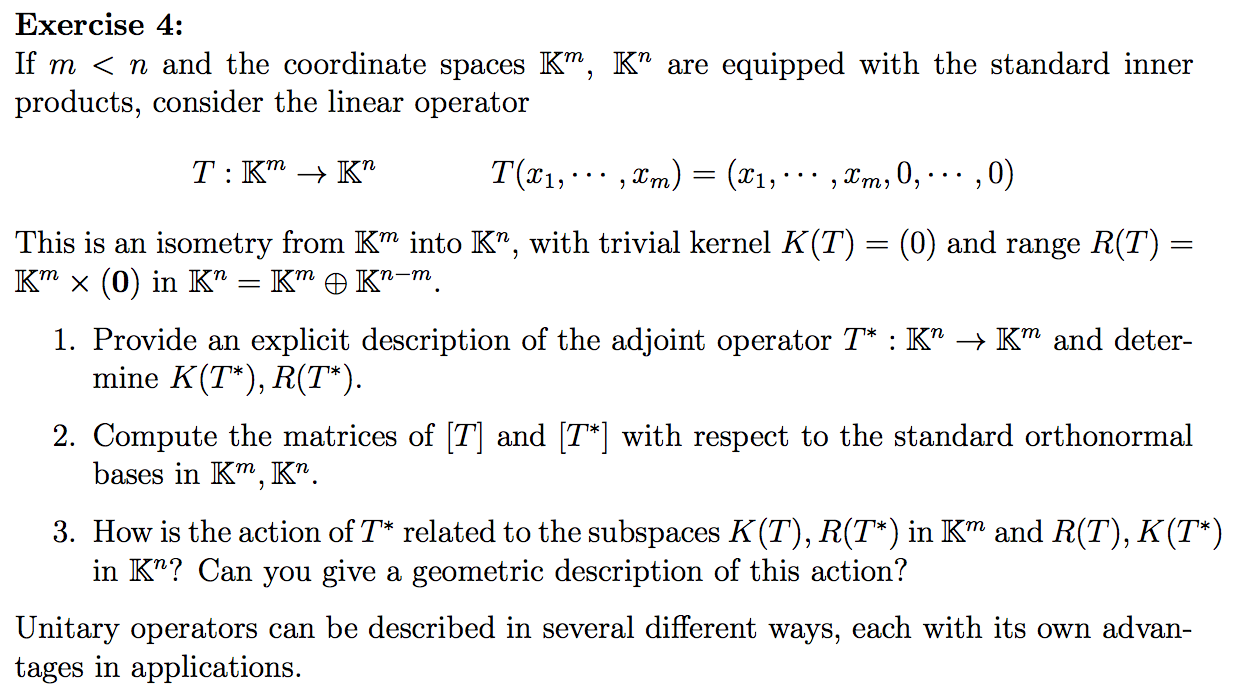
\includegraphics[width=1\textwidth]{LA-2-4.png}
\end{figure}
\end{question}
\begin{solution}
\textbf{(1)} 
Let $(e_i)$ and $(f_j)$ denote the standard bases for $\mathbb{K}^m$ and 
$\mathbb{K}^n$ respectively. Let $v \in \mathbb{K}^{n}$.
For $i = 1,2,...,m$, it follows that
\eQb
(T^* v)_i &=& (T^{*}v, e_i) \\
&=& (v,Te_i ) \\
&=& (v, f_i) \\
&=& v_i.
\eQe
Therefore, we have shown that $T^*$ is the projection onto the first $m$ coordinates.
It easily follows that $K(T^*) = (0) \times \mathbb{K}^{n-m}$ and $R(T^*) = 
\mathbb{K}^m$.

\bigskip

\textbf{(2)} $[T]$ can be written as $[I_{m\times m} ;  0_{n-m \times m}]$, and
$[T^*]$ can be written as $[I_{m \times m} 0_{m \times n-m}]$.  

\bigskip

\textbf{(3)} We can relate them as both pairs form a direct sum of $\mathbb{K}^m$,
and $\mathbb{K}^n$ respectively. Geometrically, we can describe this action as an orthogonal
projection.

\hfill $\qed$
\end{solution}

\newpage

\begin{question}[5]
\hfill
\begin{figure}[h!]
  \centering
    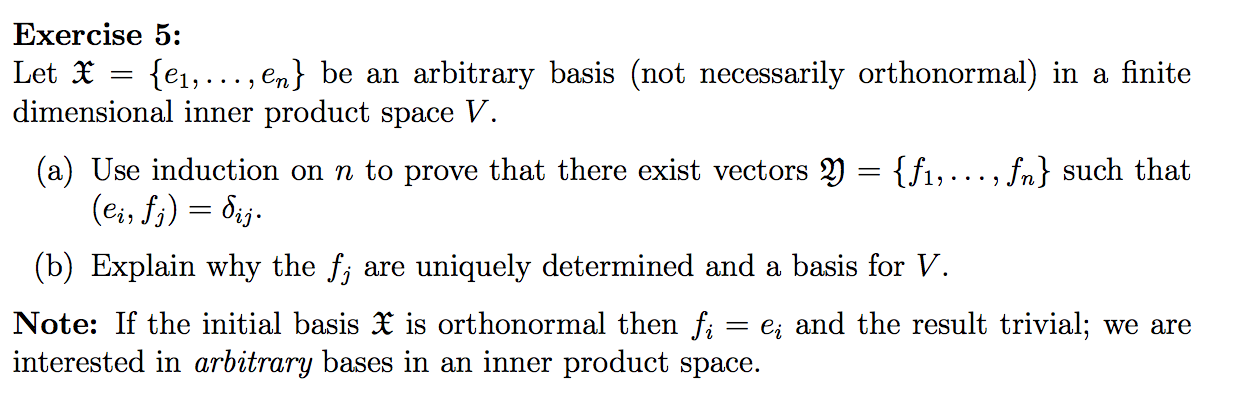
\includegraphics[width=1\textwidth]{LA-2-5.png}
\end{figure}
\end{question}
\begin{solution}  
\end{solution}

\newpage

\begin{question}[6]
\hfill
\begin{figure}[h!]
  \centering
    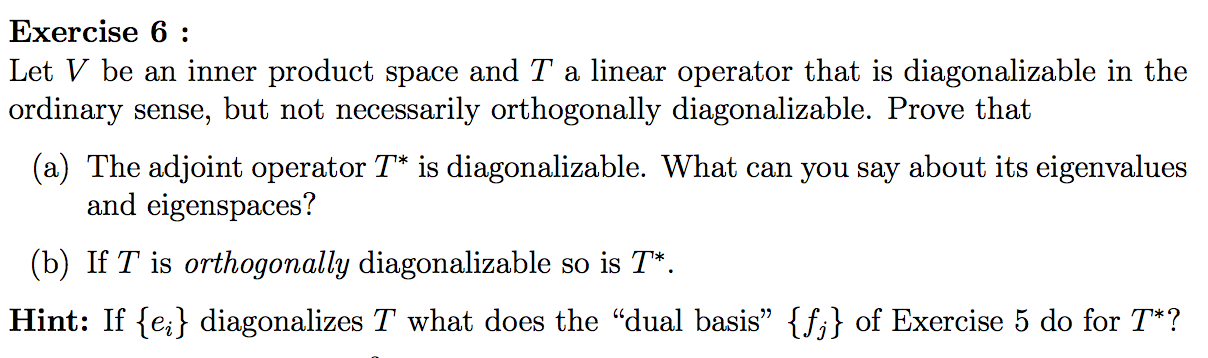
\includegraphics[width=1\textwidth]{LA-2-6.png}
\end{figure}
\end{question}
\begin{solution}
\textbf{(a)} As $T^*$ is diagonalizable, we can express $V$ as a direct sum of 
eigenspaces, which we denote as $E_{\lambda}(T^*)$ for $\lambda \in sp(T^*)$.
The same logic aapplies to $T$ being diagonalizable with $\lambda \in sp(T)$.
Hence, they will be conjugate transpose of each other, with the corrpsponding
eigenspaces. 

\smallskip

\textbf{(b)} Assume $T$ is orthogonally diagonalizable. Then, there exists an orthonormal 
basis $B$ such that $[T]_{B}$ is diagonal. As $B$ is orthonormal, we have that $[T^*]_{B}
= [T]_{B}^*$. Since a conjugate transpose of a diagonal matrix is diagonal, we see that
$[T^*]_{B}$ is a diagonal matrix. Therefore, there exists an orthonormal basis, namely $B$
such that the matrix representation of $T^*$ with respect to the orthonormal basis is diagonal.
Hence, $T^*$ is diagonalizable. 

\hfill $\qed$
  
\end{solution}

\newpage

\begin{question}[7]
\hfill
\begin{figure}[h!]
  \centering
    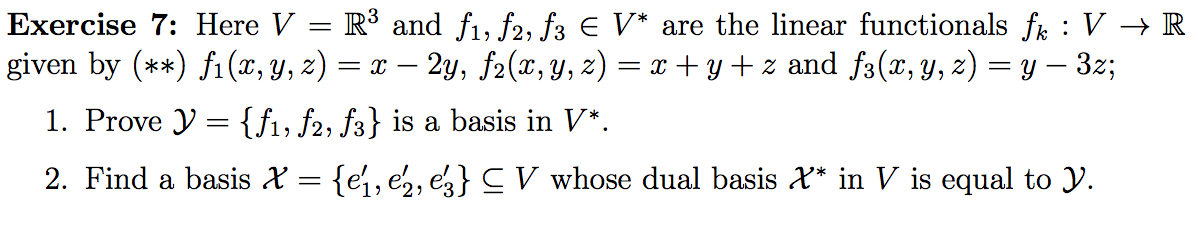
\includegraphics[width=1\textwidth]{LA-2-7.png}
\end{figure}
\end{question}
\begin{solution} 
\textbf{(1)} As the dimension of the dual space for a finite dimensional linear space 
equals the dimension of the linear space, it suffices to show that $f_1$, $f_2$, and 
$f_3$ are linearly independent. Let $\lambda_1, \lambda_2, \lambda_3 \in \mathbb{R}$, such 
that $\lambda_1 f_1 + \lambda_2 f_2 + \lambda_3 f_3 = 0$. By substitutions, it follows that
\eQb
\lambda_1 f_1(x,y,z) + \lambda_2 f_2(x,y,z) + \lambda_3 f_3(x,y,z) &=& 
\lambda_1 (x - 2y) + \lambda_2(x+y+z) + \lambda_3 (y-3z) \\
&=& (\lambda_1 + \lambda_2)x + (-2\lambda_1 + \lambda_2 + \lambda_3)y + (\lambda_2 - \lambda_3)z. \\ 
\eQe
Since the above equation holds for all $x,y,z \in \mathbb{R}$ and $\mathbb{R}$ is 
an integral domain, we obtain that
\eQb
\lambda_1 + \lambda_2 &=& 0 \\
-2\lambda_1 + \lambda_2 + \lambda_3 &=& 0 \\
\lambda_2 - \lambda_3 &=& 0 . 
\eQe
It immediately follows that $\lambda_1 = \lambda_2 = \lambda_3 = 0$. Therefore, $\mathscr{Y}$ 
is linearly independent, thus a basis in $V^*$.

\bigskip

\textbf{(2)} We wish to find vectors $v_i = (x_i, y_i, z_i)$, for $1 \leq i \leq 3$, such that
$f_i(v_j) = \delta_{ij}$. For $v_1$ we have
\eQb
x_1 - 2y_1 &=& 0 \\
x_1 + y_1 + z_1 &=& 0 \\
y_1 - 3 z_1 &=& 0. \\
\eQe
Solving the system, we obtain $x_1 = \dfrac{4}{10}$, $y_1 = \dfrac{-3}{10}$, and $z_1 = 
\dfrac{-1}{10}$. The rest can be computed in the exact same manner.
\hfill $\qed$

\end{solution}


\end{document}
